    \chapter[Neural Networks]{Neural Networks}
\label{ch:neural-networks}
Neural Networks\index{Neural Network} (NNs) are the product of various academic facets, the most prominent one being neuroscience\index{neuroscience} as the structure of a neural network mimics the computation done by the human brain, which makes use of neurons to perform complex calculations such as object recognition from visual input of the eyes. This process is very inefficient to be performed on a computer due to its computational difficulty, which is remedied by the neural network's parallel nature \cite{GURESEN2011426}. \\

The way the brain trains its neurons is through experience and thus creating a learning process, and neural networks are designed to work the same way by creating synthetic nodes which will behave like organic neurons \cite{Haykin:1994:NNC:541500}. Since this structure makes use of learnt experiences, the progress is stored in the form of weighted values at the synapse of each node. \cite{GURESEN2011426}

\section{Types of Neural Networks}

\subsection{Artificial Neural Network}\label{sec:headings}\index{headings}
An Artificial Neural Network\index{Artificial Neural Network} (ANN) (see figure~\ref{fig:annfig}) can be defined as a collection of Machine Learning\index{Machine Learning} techniques that together are able to process complex inputs into meaningful spaces or classifications without any further input from the user (such as rules) \cite{GURESEN2011426}. The ANN is a network of layers, where every node is connected to each node of the previous and next layers. A common setup for an ANN will have an input layer, hidden layer and output layer. As the ANN is traversed, an activation function is fired at each step. Activation functions\index{Activation functions} form the output behaviour of each of the neurons, by applying a specific function to the input nodes and producing a desired output \cite{Haykin:1994:NNC:541500}. The activation function may contain a numerical bias\index{bias}, which will transform its output upwards or downwards \cite{Haykin:1994:NNC:541500}. A few examples of activation functions are as follows:\\
\begin{itemize}
	
	\item\textbf{Step function}:
	\begin{marginfigure}%
		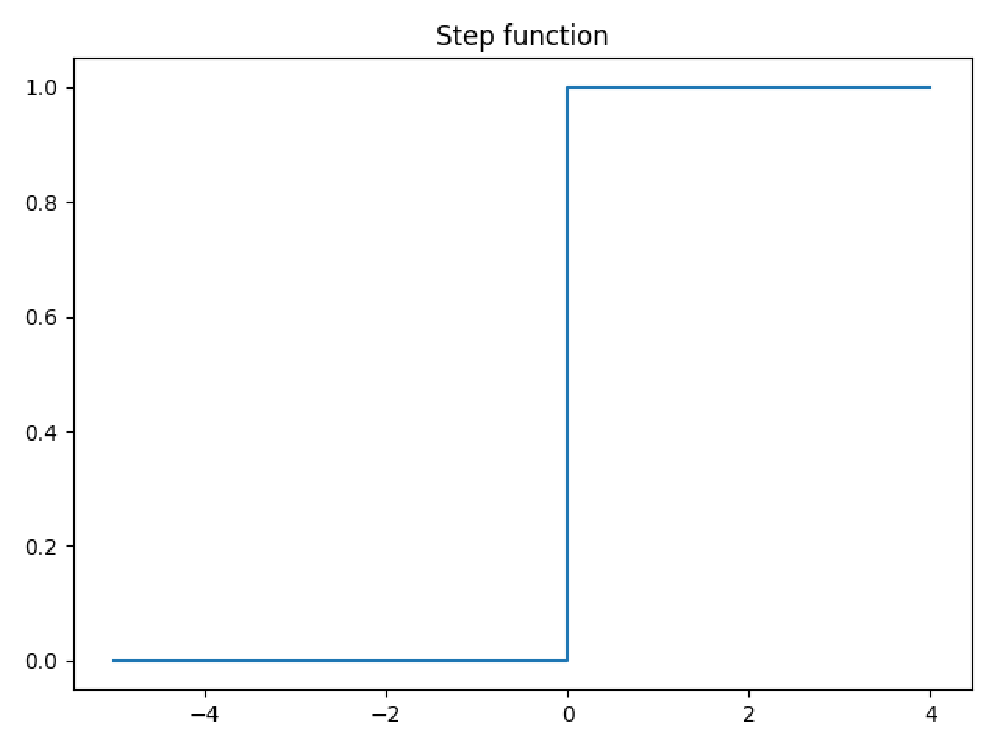
\includegraphics[width=\linewidth]{neural_network/step}
		\caption{The Step function.}
		\label{fig:stepfig}
	\end{marginfigure}
	The step function\index{step function} is also commonly called the binary function, since the output can only switch between two states: 0 or 1 \cite{sharmav_2017}. The formal definition for the graph shown in figure~\ref{fig:stepfig} is: 
	\begin{equation}
	\begin{cases}
	1 & \text{if $x < 0 $} \\
	0 & \text{otherwise}
	\end{cases}
	\end{equation} 
	A problem with this step function is the steep change from 0 to 1, which could cause the output to become inaccurate as values which are close to 0 but have different signs (negative and positive) will have a massive discrepancy although being close to each other, and values which are further away from the threshold will have the same effect as if they were close.
	
	\item\textbf{Sigmoid function}:
	\begin{marginfigure}%
		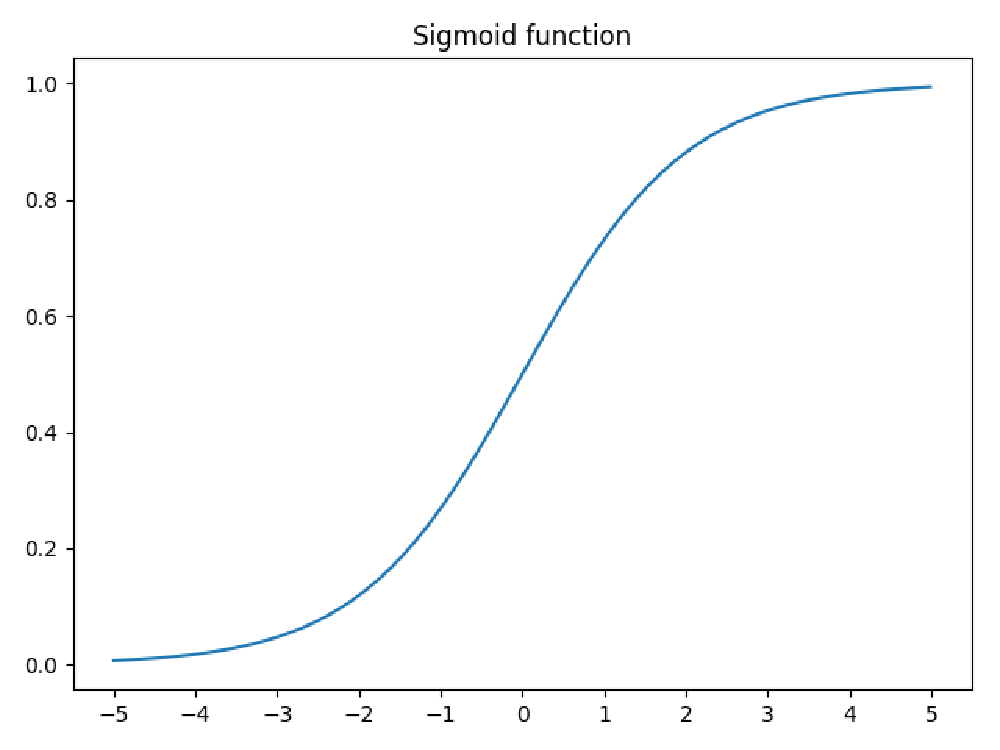
\includegraphics[width=\linewidth]{neural_network/sigmoid}
		\caption{The sigmoid function.}
		\label{fig:sigfig}
	\end{marginfigure} The Sigmoid function\index{sigmoid function} is an improvement over the step function as it smoothens out the steep change between the two states. This function maps the input to a value between 0 and 1, both ends being an asymptote\index{asymptote}. The Sigmoid function shown in figure~\ref{fig:sigfig} is as follows \cite{Haykin:1994:NNC:541500, sharmav_2017}: $$f(x) = \frac{1}{1+e^{-x}}$$
	
	\item\textbf{Hyperbolic Tangent function}:
	\begin{marginfigure}%
		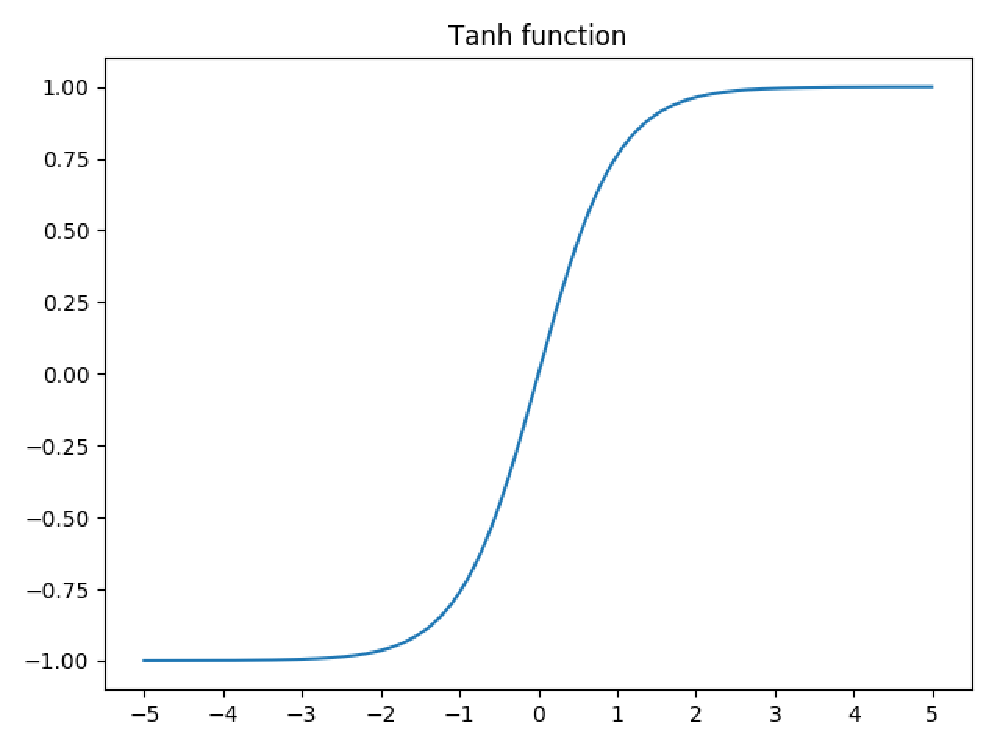
\includegraphics[width=\linewidth]{neural_network/Tanh}
		\caption{The Tanh function.}
		\label{fig:tanhfig}
	\end{marginfigure}
	The Hyperbolic Tangent function\index{Hyperbolic Tangent function}\index{Tanh} (Tanh) is very similar to the Sigmoid function, with a more stable gradient and an asymptotic range between -1 and 1, thus including negative values \cite{Haykin:1994:NNC:541500,sharmav_2017}. The function shown in figure~\ref{fig:tanhfig} is the following \cite{sharmav_2017}: $$tanh(x) = \frac{2}{1+e^{-2x}}-1 $$
	
\end{itemize}
The traversal goes from input nodes to the output nodes, and the output will be a mapped function of the input, firing activation functions\index{activation function} at each step \cite{GURESEN2011426, sharmav_2017}.\\ Before performing any predictions, the ANN needs to be trained with labelled data in order to adjust the synapses to their optimal values to form the mapping. \\ The goal of the learning process is to minimize the output of a cost function\index{cost function}, taking into consideration the error value \cite{Haykin:1994:NNC:541500}. Each time the input is fed forward through the network, the error of the predicted output is compared to the actual output and thus produce an error value. The cost function $C(n)$, in terms of error $e_k(n)$ is defined as $C(n) = \frac{1}{2}e^2_k(n)$ \cite{Haykin:1994:NNC:541500}. This error needs to be minimized, which is done through backpropagation\index{backpropagation}, which is the process where the biases are updated by distributing the error from the layer closest to the output inwards, applying the derivative of the activation function in the process \cite{doi:10.1080/02626669809492102}.\\ The error delta in terms of weight $w_{kj}$ is calculated with the following formula: $\Delta w_{kj}(n) = \alpha e_k(n)x_j(n)$ where $\alpha$ is the learning rate\index{learning rate}, $e_k(n)$ is the error and $x_j(n)$ is the input \cite{Haykin:1994:NNC:541500}. The synapses are updated by adding the calculated delta to the weight, formally, $w_{kj}(n+1) = w_{kj}(n) + \Delta w_{kj}(n)$ where $w_{kj}(n)$ is the previous weight and $\Delta w_{kj}(n)$ is the calculated weight difference \cite{Haykin:1994:NNC:541500}.\\ Techniques such as gradient descent are used to converge the weights to a minimum error value at a specified rate of change, called the learning rate \cite{doi:10.1080/02626669809492102}.\\ As the ANN performs epochs, the error of the synapses will converge towards the optimal value, which once reached, the model will be trained. Once the model is trained, one can perform predictions by passing an input through the network and observing the output.
\begin{figure}
	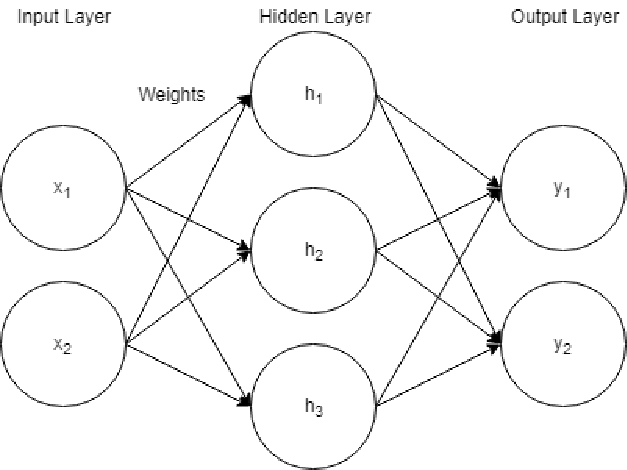
\includegraphics{neural_network/ANN}
	%  \checkparity This is an \pageparity\ page.%
	\caption[ANN][6pt]{This diagram is a visual representation of an ANN.}
	\label{fig:annfig}
	%\zsavepos{pos:annfig}
\end{figure}

\subsection{Convolutional Neural Network}\label{sec:headings}\index{headings}
A Convolutional Neural Network (CNN)(see figure~\ref{fig:cnnfig})\index{Convolutional Neural Network} is a variant of ANN and are commonly used for image processing and recognition. A CNN usually is a multi-layered network, where each layer will apply a specific function to an image \cite{NIPS2012_4824, karpathy_2018}. A CNN can use different kinds of layers, each with their own function and output, for example:
\begin{itemize}
	\item\textbf{Features\index{Feature}}: The images are reduced to similar patterns, where each pattern is a small subset of the image and is present in both images \cite{rohrer_2016}.
	\item\textbf{Convolutions}: A filter is applied across every pixel to calculate the similarity between the filter (also referred to as a kernel) and the sample with a convolution function\index{Convolution} \cite{rohrer_2016}. This will output a value that represents the likeness of the feature to the image; the higher the number, the higher the similarity \cite{rohrer_2016}.
	\item\textbf{Average/Max Pooling}: This process\index{Pooling} shrinks the images while still keeping its important features \cite{rohrer_2016}. A small window which is typically 2x2 iterates over pixels \cite{karpathy_2018}, stepping a specific number of pixels each time to possibly avoid overlapping calculations \cite{Ciresan:2011:FHP:2283516.2283603}. The output of this filter is the maximum or average value inside the window \cite{rohrer_2016}. Pooling greatly helps to reduce the computational overhead of processing a large number of pixels and thus converge in less time \cite{Ciresan:2011:FHP:2283516.2283603}.
	\item\textbf{Rectified Linear Units}: A Rectified Linear Unit\index{Rectified Linear Unit} (ReLU) is considered as an activation function, in that the output is filtered to contain only positive values \cite{sharmav_2017}. This function sets all negative values to 0 and ignores positive ones \cite{sharmav_2017, rohrer_2016}. This is used to prevent learned values from lingering close to 0 or becoming such a large negative number that it will inhibit the performance \cite{rohrer_2016}. Formally \cite{karpathy_2018},
	\begin{equation}
	\begin{cases}
	x & \text{if $x > 0 $} \\
	0 & \text{otherwise}
	\end{cases}
	\end{equation} 
	\item\textbf{Fully-Connected Layer}: A fully-connected layer\index{Fully-Connected Layer} (FC) treats the input as a singular list of nodes \cite{rohrer_2016} where each node is connected to all the previous nodes \cite{karpathy_2018}. Each node contains a weighted value which determines the contribution to a specific category when the node is fired \cite{rohrer_2016}. When the layer is activated, the nodes go through a voting process, where each node will vote to which category the input image falls under \cite{rohrer_2016}. The weights will determine which nodes will have more impact in the voting process, and the category with the bigger value of votes will classify the image \cite{rohrer_2016, karpathy_2018}.
	
	\begin{figure}[h]
		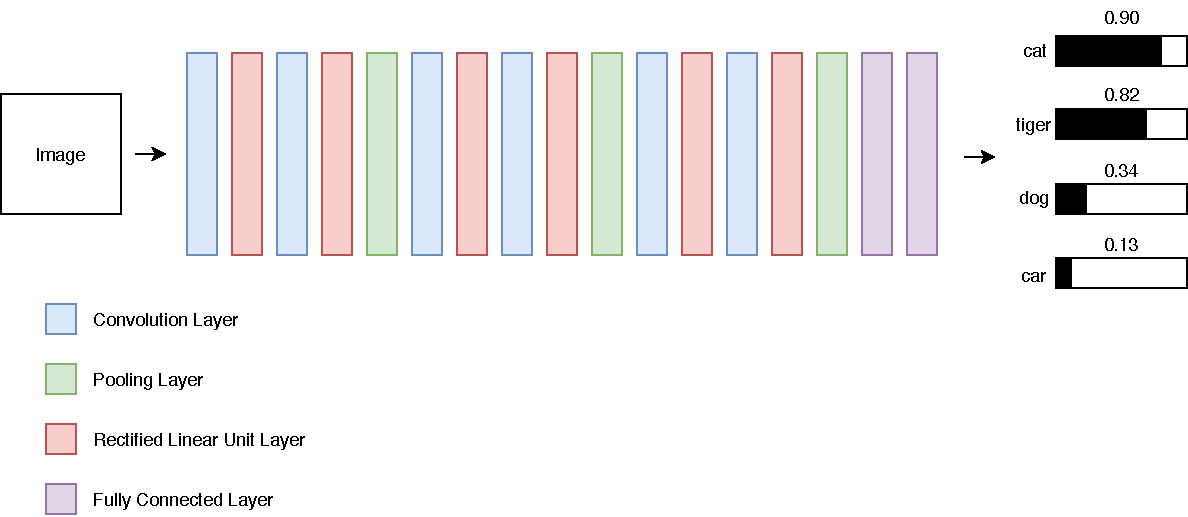
\includegraphics[width=\linewidth]{neural_network/CNN}%
		\caption{A diagram of a CNN with deep learning.}%
		\label{fig:cnnfig}%
	\end{figure}
\end{itemize}

A CNN can have multiple repetitions of a set of layers, which will form a deep learning\index{deep-learning} model with a multitude of layers that will eventually produce a final classification of the image \cite{NIPS2012_4824, DBLP:journals/corr/KalchbrennerGB14}. Training of a CNN occurs by feeding the network labelled data and adjusting the weights and features during a backpropagation\index{backpropagation} step, distributing the error and converging to a set error threshold, similar to how ANNs perform their training \cite{DBLP:journals/corr/KalchbrennerGB14,rohrer_2016,karpathy_2018}.
